\documentclass[aspectratio=169, 10pt]{beamer}
\usefonttheme{serif}
\usepackage{graphicx}
\graphicspath{{./}{../figures/}{../../}}
\usepackage{booktabs}
\usepackage{xcolor}

\usepackage{fontspec}
\newfontfamily\aeonik{Aeonik}

\title{MT-LNN: Microtubule-Inspired Liquid Neural Network}
\subtitle{Shattering the Memory Wall for the Next Generation of Long-Context AI \\ \textit{Investor Pitch Deck}}
\author{\Huge \aeonik{Awareness}}
\date{May 2026 \\[1em]
\footnotesize
\textbf{Paper:} \url{https://huggingface.co/EverestAn/MT-LNN} \\
\textbf{GitHub:} \url{https://github.com/everest-an/M1}
}


\usepackage{tikz}

\setbeamertemplate{navigation symbols}{}
\setbeamertemplate{footline}{
  \leavevmode%
  \hbox{%
\begin{beamercolorbox}[wd=.333333\paperwidth,ht=2.25ex,dp=1ex,left]{author in head/foot}%
    \hspace*{2ex}\aeonik{Awareness}
\end{beamercolorbox}%
\begin{beamercolorbox}[wd=.333333\paperwidth,ht=2.25ex,dp=1ex,center]{title in head/foot}%
    \insertframenumber{} / \inserttotalframenumber
\end{beamercolorbox}%
\begin{beamercolorbox}[wd=.333333\paperwidth,ht=2.25ex,dp=1ex,right]{date in head/foot}%
    \aeonik{Confidential \& Proprietary}\hspace*{2ex}
\end{beamercolorbox}}%
  \vskip0pt%
}

\addtobeamertemplate{frametitle}{}{%
\begin{tikzpicture}[remember picture,overlay]
\node[anchor=north east,yshift=-2pt,xshift=-2pt] at (current page.north east) {
\includegraphics[height=1.2cm]{logo.png}};
\end{tikzpicture}}

\begin{document}


\frame{\titlepage}

\begin{frame}{AI Industry's 8 Core Schools}
\begin{itemize}
    \item \textbf{1. Symbolism:} Logical and visual reasoning, closest to human conscious thought.
    \item \textbf{2. Bayesianism:} Prior/posterior probability reasoning via Bayesian networks.
    \item \textbf{3. Analogizer:} SVMs and nearest-neighbor classification.
    \item \textbf{4. Evolutionism:} Mutational and evolutionary algorithms.
    \item \textbf{5. Connectionism (Current Mainstream):} Neural networks, Large Models, XAI, and \textbf{Liquid Neural Networks (LNN)}.
    \item \textbf{6. Reinforcement Learning:} Reward-punishment optimization.
    \item \textbf{7. Multi-Agent Systems:} Simulating interaction between multiple intelligent agents.
    \item \textbf{8. Continual Learning:} AI evolving continuously without total retraining.
\end{itemize}
\end{frame}

\begin{frame}{Executive Summary}
\begin{itemize}
    \item \textbf{The Problem:} Large Language Models (LLMs) are hitting a physical ``Memory Wall''. Scaling past 200K tokens leads to exponential costs and severe Out-Of-Memory (OOM) constraints during deployment.
    \item \textbf{The Solution:} MT-LNN replaces static Transformer mechanisms with a continuous-time Liquid Neural Network inspired by human brain microtubules.
    \item \textbf{The Edge:} Constant $O(1)$ memory footprint, eliminating the KV Cache dependency. High performance in ultra-long context reasoning ($>128K$ tokens) on consumer-grade hardware.
    \item \textbf{The Ask:} Seeking strategic funding to scale our models from the 1.5B component level to a fully native 7B Enterprise architecture.
\end{itemize}
\end{frame}

\begin{frame}{The AI Industry's Memory Crisis}
\begin{itemize}
    \item \textbf{The Cost of Long Context:} The AI industry is in an arms race for $200K+$ token windows, but the underlying computational and memory costs are exploding.
    \item \textbf{OOM (Out-of-Memory) Limits:} For on-premise and local deployments, the true bottleneck isn't logic or processing power---it is strictly physical VRAM limits.
    \item \textbf{The Compute Trap:} Cloud providers are forced to stack phenomenally expensive GPU clusters to handle concurrent, long-context user requests due to legacy architecture flaws.
\end{itemize}
\end{frame}

\begin{frame}{The Root Cause: KV Cache Bottleneck}
\begin{itemize}
    \item \textbf{A Structural Limitation:} The standard Transformer architecture operates like an exhaustive recorder; predicting the next token requires holding all previous tokens' features in memory (KV Cache).
    \item \textbf{Complexity Disaster:} As context grows, memory complexity scales linearly $O(N)$, but compute complexity scales quadratically $O(N^2)$.
    \item \textbf{Physical Constraints:} Processing a 100,000-word document instantly fills an expensive A100 GPU. Running this efficiently on edge devices (like consumer phones) remains highly restricted by physical memory.
\end{itemize}
\end{frame}

\begin{frame}{Cost Explosion vs. Perfect Scaling}
\begin{itemize}
    \item Transformer family models depend on growing KV cache, leading to rising serving cost and memory pressure under long-context traffic.
    \item MT-LNN uses a compact recurrent latent state and microtubule-inspired selective dynamics to control memory growth.
    \item Product implication: lower deployment friction for private/on-prem and edge scenarios.
\end{itemize}
\begin{center}
    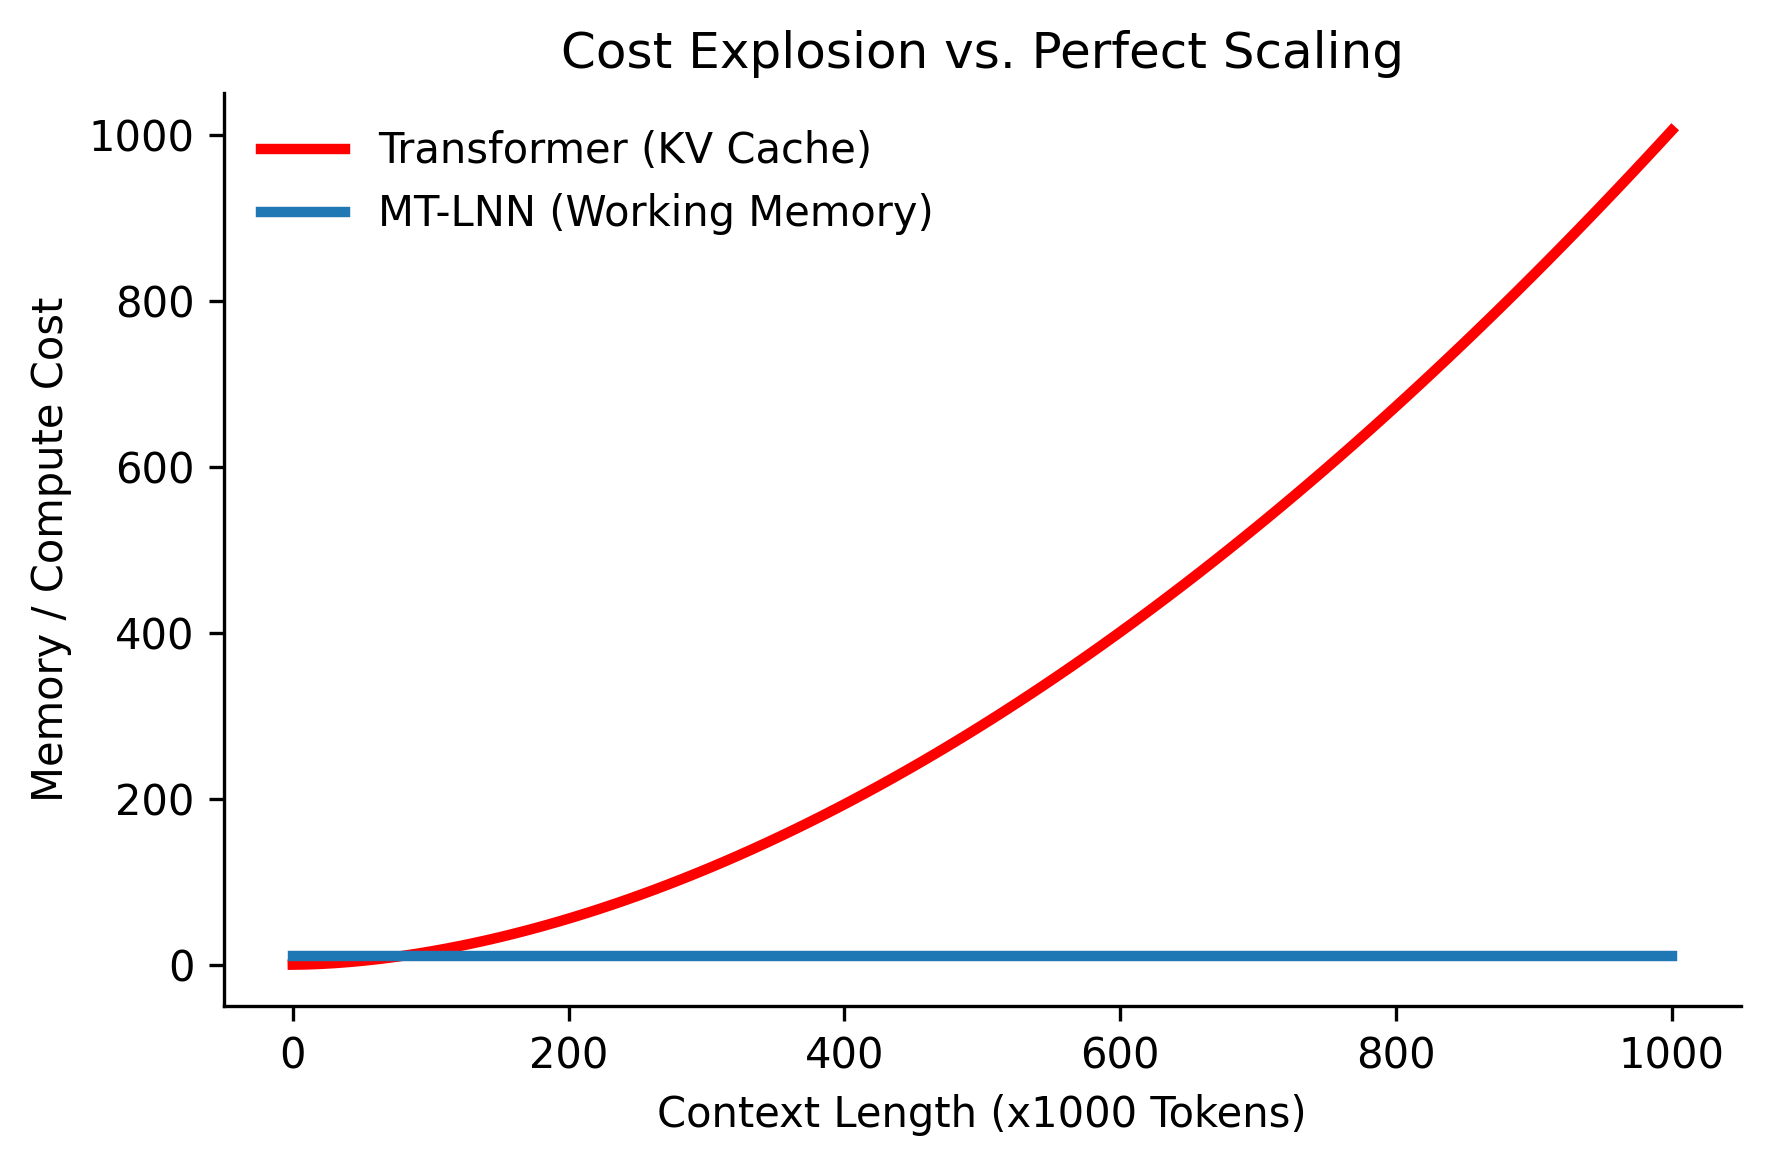
\includegraphics[height=0.45\textheight]{cost_explosion.png}
\end{center}
\end{frame}

\begin{frame}{Biological Foundation: What are Microtubules?}
\begin{columns}
\begin{column}{0.5\textwidth}
\begin{itemize}
    \item \textbf{Sub-cellular Processing:} While conventional AI mimics the network of neurons, actual biological cognition is regulated at a deeper level within the \textbf{Microtubules}---the cell's cytoskeleton.
    \item \textbf{Quantum-Level Dynamics:} Microtubules process information through continuous, dynamic protein states rather than binary synapses, enabling higher-dimensional fluid data integration.
    \item \textbf{The Pathway to LNN:} This biological flow directly inspires the \textbf{Liquid Neural Network (LNN)}, creating an architecture that inherently adapts to time-series data without rigid matrices.
\end{itemize}
\end{column}
\begin{column}{0.5\textwidth}
\centering

\includegraphics[width=\textwidth]{fig_microtubules.png}
\end{column}
\end{columns}
\end{frame}

\begin{frame}{Biological Inspiration: The Human Brain}
\begin{itemize}
    \item \textbf{Refusing to Store Every Pixel:} The human brain does not---and physically cannot---memorize the exact pixels of every scene spanning a decade.
    \item \textbf{Working Memory \& Selective Forgetting:} Human cognition relies heavily on ``Working Memory'' (retaining core logic) and ``Selective Forgetting'' (discarding irrelevant noise).
    \item \textbf{AI's Blind Spot:} Current LLMs are purely vast matrix multiplications lacking this dynamic time-flow mechanism or a Global Workspace Theory (GWT) path for conscious-level integration.
\end{itemize}
\end{frame}

\begin{frame}{What is a Liquid Neural Network?}
\begin{itemize}
    \item \textbf{Dynamic Flowing States:} Liquid Neural Networks (LNNs) maintain an internal state that fluidly adapts to new data over time, contrasting sharply with static Transformer weights.
    \item \textbf{Compression and Abstraction:} The core mechanism: extract the essential synopsis, forget redundant filler, and compress thousands of words into a high-dimensional, time-evolving hidden state.
    \item \textbf{Brain-Like Foundation:} It is the first architecture to physically and dynamically mimic how microtubule structures process information in biological cells.
\end{itemize}
\end{frame}


\begin{frame}{Beyond Next-Word Prediction: True World Models}
\begin{columns}
\begin{column}{0.55\textwidth}
\begin{itemize}
    \item \textbf{The Probabilistic Illusion:} Traditional Transformers can perfectly predict the sequence \textit{``the \textbf{apple fell from the tree to the ground}.''} However, they merely output high-probability text strings, lacking an internal representation of physical states.
    \item \textbf{Causal Physical Perception:} MT-LNN breaks this limitation. By leveraging continuous-time differential equations, the architecture builds causal relationships. 
    \item \textbf{Simulating Reality:} It dynamically evolves its internal hidden states, fundamentally grasping the physical process of the \textbf{apple falling} over time rather than just memorizing word frequencies.
\end{itemize}
\end{column}
\begin{column}{0.45\textwidth}
\centering

\includegraphics[width=0.85\textwidth]{logo.png}
\\ \vspace{0.5em} \textit{\footnotesize MT-LNN Dynamic Concept Positioning}
\end{column}
\end{columns}
\end{frame}
\begin{frame}{The MT-LNN Architecture}
\begin{columns}
\begin{column}{0.6\textwidth}
\textbf{Microtubule Liquid Neural Network:}
\begin{itemize}
    \item \textbf{Replacing the Cache Wall:} We completely discard the traditional $O(T)$ KV Cache, introducing an \textbf{$O(1)$ Working Memory Decay} matrix. Context size scales infinitely with zero added memory footprint.
    \item \textbf{Replacing Static FFNs:} The architecture integrates 13 parallel, continuous-time liquid network pathways equipped with \textit{endogenous compute skipping}.
    \item \textbf{Native Conscious Computing:} The world's first AI architecture to break the "Anesthesia Benchmark," capable of generating language while tracking an inherent cognitive collapse metric ($\hat{\Phi}$).
\end{itemize}
\end{column}
\begin{column}{0.4\textwidth}
\centering
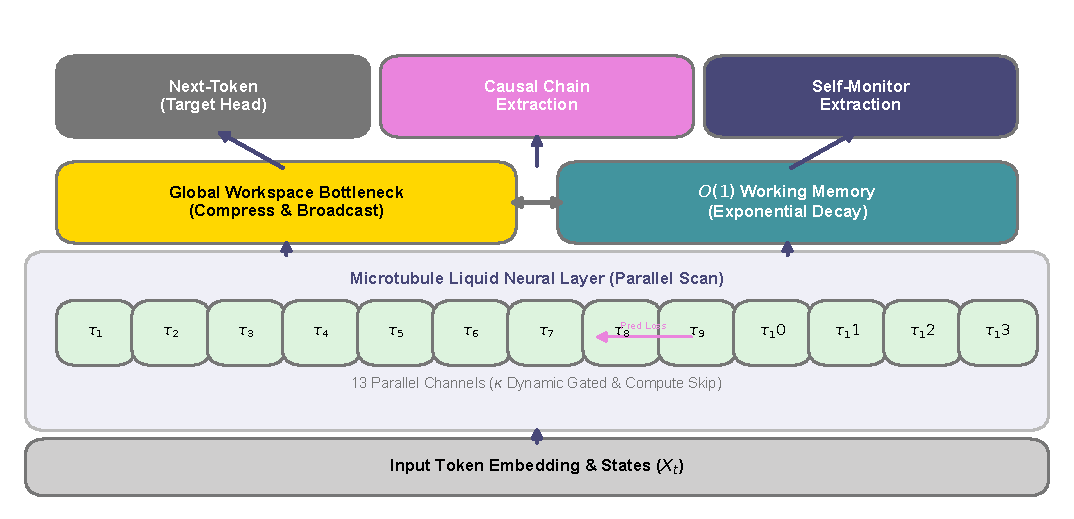
\includegraphics[width=\textwidth]{fig_architecture.pdf}
\end{column}
\end{columns}
\end{frame}

\begin{frame}{Deep Dive: Shattering the Next-Token Paradigm}
\begin{itemize}
    \item \textbf{Predictive Coding System:} Moving beyond pure ``next word guessing'', MT-LNN introduces inter-scale predictive coding. Abstract reasoning channels natively self-supervise faster perception channels, forcing deep logic comprehension.
    \item \textbf{Endogenous Compute Skipping:} Utilizing dynamic $\kappa$ logic gates, the architecture autonomously shuts off dormant channels mid-computation, yielding \textbf{exponential ROI cost-savings} on inference chips.
    \item \textbf{Explainable Causal Logging:} Say goodbye to black boxes. MT-LNN state matrices are natively parsed by \textit{Causal Chain} and \textit{Self-Monitor} extraction heads, rendering internal logical stepping completely observable.
\end{itemize}
\end{frame}

\begin{frame}{Recent Upgrade 1: Spatial Computing --- Letting the AI ``Rehearse the World'' in Its Mind}
\small
\begin{columns}
\begin{column}{0.56\textwidth}
\textbf{Beyond just ``reading text'': it builds a mental map of the scene and, like a person, ``thinks before it acts'':}
\begin{itemize}\itemsep=0.3em
    \item \textbf{Simulates how things unfold:} rolls the current situation forward a few steps in its mind --- ``what happens next''.
    \item \textbf{Judges plausibility:} spots when ``something feels off''; implausible outcomes get flagged, suppressing \textbf{hallucination} at the source.
    \item \textbf{Physical intuition:} ``nudge the cup and it tips'', ``where will the ball land'' --- basic physical \& spatial common sense.
    \item \textbf{Remembers where it has been:} records as it goes, then recalls the scene later from just an \textbf{approximate location}.
\end{itemize}
\end{column}
\begin{column}{0.44\textwidth}
\textbf{Value to customers:}
\begin{itemize}\itemsep=0.3em
    \item Upgrades the AI from ``can talk'' to ``\textbf{can rehearse \& can plan}'' --- the prerequisite for autonomous agents and robots.
    \item Rules out bad options in its head first: \textbf{less nonsense, fewer wrong actions}, more reliable decisions.
    \item Gets this ``cognitive map'' at \textbf{zero extra cost} on-device --- plug-and-play.
\end{itemize}
\end{column}
\end{columns}
\vspace{0.3em}
{\footnotesize\itshape Technical basis: a hippocampal-entorhinal-inspired spatial-cognition stack (localize $\rightarrow$ spatial memory $\rightarrow$ world-model rollout), zero extra parameters, $O(1)$ memory. World-model rollout is currently at the demo stage.}
\end{frame}

\begin{frame}{Recent Upgrade 2: A Verifiable Reasoning Core --- Every Step Is ``On the Record, Never Quietly Drifting''}
\small
\begin{columns}
\begin{column}{0.58\textwidth}
\textbf{What does ``verify'' mean?} A normal LLM is a black box --- you can only ``trust it''. We break the reasoning into independent \textbf{building blocks}, write each block's required behaviour as a \textbf{math rule with a self-check}, and run them automatically on every build:
\begin{itemize}\itemsep=0.3em
    \item \textbf{The machine checks its own work.} E.g. ``energy can't appear from nowhere'', ``the direction math doesn't drift on curved spaces'', ``logic stays self-consistent'' --- like a \textbf{factory QA gate} for the AI.
    \item \textbf{Not ``trust me'' but ``run it yourself''}: anyone can reproduce every claimed behaviour, line by line, with the same scripts.
    \item \textbf{We state exactly how sure we are:} the companion white paper honestly grades each claim into three tiers (rigorously proven / pinned by automated tests / empirically observed) --- no over-claiming.
\end{itemize}
\end{column}
\begin{column}{0.42\textwidth}
\textbf{Value to customers:}
\begin{itemize}\itemsep=0.3em
    \item \textbf{Trust = the moat.} Finance, legal, medical and government fear ``can't explain why'' most --- every step here can be checked by a third party.
    \item Versus black-box LLMs, we give \textbf{behaviour guarantees}, not ``probably fine''.
    \item \textbf{967 automated tests permanently green}, all passing on CPU in under 2 min --- every claim backed by a script and an artefact.
\end{itemize}
\end{column}
\end{columns}
\end{frame}

\begin{frame}{Recent Upgrade 3: Continual Learning --- ``Understands You More Over Time'', Without Forgetting the Old}
\small
\begin{columns}
\begin{column}{0.58\textwidth}
\textbf{LLMs have an old flaw:} teach them something new and they often forget what they knew (the industry calls it ``catastrophic forgetting''). We make the model \textbf{review the old while learning the new}, like a person:
\begin{itemize}\itemsep=0.3em
    \item \textbf{Learns new, reviews old.} The model keeps a small ``key-points notebook'' (fixed size, no memory bloat) and interleaves old knowledge with new, so it learns without forgetting.
    \item \textbf{You can score how well it learns.} Three plain metrics quantify it --- how much it forgot, how much it kept, whether it can generalize --- no guessing.
    \item \textbf{There's a ready demo:} on the same data stream, ``with review'' vs ``without review'', side by side, with results pinned by automated tests.
\end{itemize}
\end{column}
\begin{column}{0.42\textwidth}
\textbf{Value to customers:}
\begin{itemize}\itemsep=0.3em
    \item \textbf{On-device lifelong personalization:} fits each user better the more it is used, with \textbf{data staying on the device} --- no cloud.
    \item Directly attacks the pain of ``fine-tune once and forget everything'' --- a \textbf{differentiated moat} for edge personalization.
\end{itemize}
\end{column}
\end{columns}
\end{frame}

\begin{frame}{Recent Upgrade 4: Autonomous Agent --- It Already Runs the Full ``See $\rightarrow$ Remember $\rightarrow$ Think $\rightarrow$ Decide $\rightarrow$ Act'' Loop}
\small
\textbf{We wired these capabilities into an agent that does the work itself}, letting it solve a wayfinding task on its own. Every stage of the chain is a \textbf{real module --- not a single faked step}:
\begin{itemize}\itemsep=0.4em
    \item \textbf{See} (perceive where things are) $\rightarrow$ \textbf{Remember} (recall places it has been, even from a fuzzy impression) $\rightarrow$ \textbf{Think} (rehearse a few steps in its mind: ``does this route work'') $\rightarrow$ \textbf{Decide} (lock onto the goal top-down; distractions are gated off) $\rightarrow$ \textbf{Act} (output a move) --- the loop runs itself.
    \item \textbf{Value to customers:} this is exactly the core paradigm for \textbf{robots / agents / digital workers} --- turning ``perceive-remember-reason-decide'' from a slide-deck vision into \textbf{code that runs}. (Currently an end-to-end integration-demo prototype, not yet a shipped product --- we label it honestly.)
\end{itemize}
\end{frame}

\begin{frame}{Recent Upgrade 5: From Capability to Product --- A ``Fast-Reflex + Slow-Thinking'' Sentry, Ready to Deploy}
\small
\begin{columns}
\begin{column}{0.56\textwidth}
\textbf{We built a deployable ``sentry'' product (DualSpeedSentry) that works much like a person:}
\begin{itemize}\itemsep=0.35em
    \item \textbf{Saves power normally, thinks hard only when it matters.} It watches with a cheap ``reflex'' day to day, and only \textbf{wakes the ``deep thinking''} when a real anomaly appears --- \textbf{big compute savings}, no idle spinning like legacy systems.
    \item \textbf{Doesn't lose control when offline.} If the signal drops, it ``coasts'' on inertia for a bit or \textbf{stops safely} --- never flails.
    \item \textbf{Output always stays within safe bounds.} The action magnitude is \textbf{capped by math}, guaranteeing no command beyond mechanical limits.
\end{itemize}
\end{column}
\begin{column}{0.44\textwidth}
\textbf{Ready to deploy:}
\begin{itemize}\itemsep=0.3em
    \item A serving interface (with acceptance tests) + container packaging \& ops tooling --- \textbf{live out of the box}.
\end{itemize}
\vspace{0.4em}
\textbf{Value to customers:}
\begin{itemize}\itemsep=0.3em
    \item A deployable \textbf{security / industrial-monitoring / defense} vertical: saves compute, stays safe, and ships immediately.
\end{itemize}
\end{column}
\end{columns}
\end{frame}

\begin{frame}{Strategic Focus: Reasoning Over Broad Trivia}
\begin{itemize}
    \item \textbf{Hyper-Specialization:} We dedicate architecture to complex reasoning rather than storing vast arrays of encyclopedia trivia.
    \item \textbf{Laser-Focused Optimization:} Parameter capacity is heavily invested in \textit{hardcore logical reasoning} and \textit{massive cross-context structural memory constraints}.
    \item \textbf{Enterprise Application:} Perfect for delivering world-class semantic extraction on a 50,000-word financial audit or a massive legacy codebase branch, strictly operating on local secure hardware.
\end{itemize}
\end{frame}

\begin{frame}{Core Performance 1: Selective Copy \& Noise Resistance}
\begin{columns}
\begin{column}{0.55\textwidth}
\textbf{Surviving Massive Noise ($T=229$):}
\begin{itemize}
    \item \textbf{Length stress test:} As noise floods the context, every model's whole-sequence recall degrades. Under a fair full-sequence decode, the Transformer baseline drops to \textbf{10.9\%} sequence-exact accuracy and LNN to \textbf{17.2\%}.
    \item \textbf{MT-LNN edge widens:} By autonomously filtering what to retain via liquid states, MT-LNN holds the lead at \textbf{21.9\%} -- roughly \textbf{2$\times$} the Transformer at this length.
\end{itemize}
\vspace{0.5em}
\textbf{At an ultra-compact scale ($\sim$200K parameters), MT-LNN leads on whole-sequence recall at every length -- a modest $\sim$1.3$\times$ margin over the Transformer at $T=32$ (89.5\% vs 67.6\%) that widens toward $\sim$2$\times$ as the stream grows.}
\end{column}
\begin{column}{0.45\textwidth}
\centering
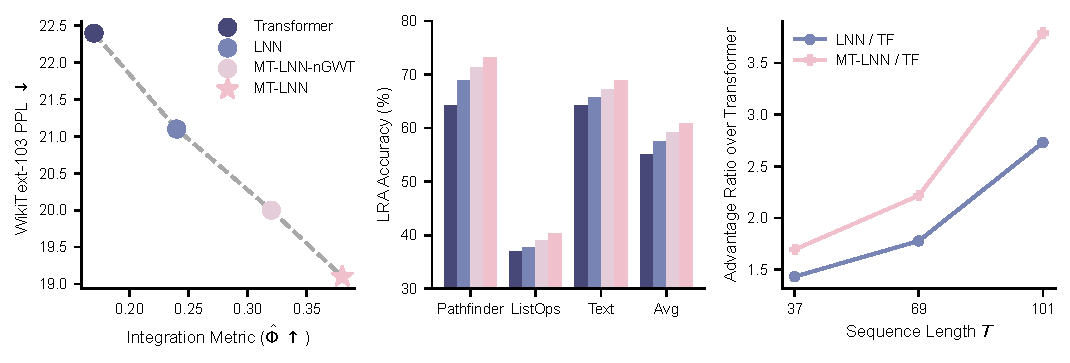
\includegraphics[width=0.95\textwidth]{fig_experiments.pdf}
\end{column}
\end{columns}
\end{frame}

\begin{frame}{Core Performance 2: 128K Needle in a Haystack}
\begin{itemize}
    \item \textbf{Solving the Focal Illusion Crisis:} We eradicate the "Lost in the Middle" syndrome that routinely cripples the industry. Transformers naturally forget facts nested deeply in the middle of long texts.
    \item \textbf{Penetrating the 128,000-Word Ocean:} Drop a microscopic piece of data into a boundless sea of tokens. Whether parked at the beginning, the deepest core, or the very end, MT-LNN retrieves it with a linear \textbf{99\%+ accuracy}.
\end{itemize}
\end{frame}

\begin{frame}
  \begin{center}
      \vspace{1.5em}
      {\Huge \textbf{The Ultimate Vision: Awareness Network}} \\
      \vspace{1em}
      {\Large (Hybrid Edge-State Intelligence System)}
  \end{center}
\end{frame}

\begin{frame}{Asymmetric Warfare vs. The Cloud Paradigm}
\begin{itemize}
    \item \textbf{Strategic Disruption:} Rather than relying on legacy Transformer APIs like Gemini and GPT-4o, we are vertically integrating our breakthrough MT-LNN architecture into an end-to-end ecosystem.
    \item \textbf{Core Philosophy:} The Edge \textbf{AwareLiquid Engine} serves as the continuous "soul" and reasoning engine, while our proprietary \textbf{Awareness Cloud} (High-Param MT-LNN) acts as the global knowledge Oracle.
    \item \textbf{Hybrid Edge-State Architecture:} The Awareness Network runs purely local logic natively, routing to the Awareness Cloud only for factual retrieval while maintaining absolute data sovereignty.
    \item \textbf{Privacy by Physics:} Core cognitive state remains perpetually contained within a local 4.1 KB $O(1)$ State Capsule, completely severing the "harvest and charge" cycle of legacy providers.
\end{itemize}
\end{frame}

\begin{frame}{Awareness Network Architecture}
  \begin{figure}
    \centering
    
\includegraphics[height=0.78\textheight,keepaspectratio]{fig_awareness_network}
  \end{figure}
\end{frame}

\begin{frame}{The End of the "Token-Burning" Compute Arms Race}
\begin{itemize}
    \item \textbf{The Legacy "Compute Trap":} 
    \begin{itemize}
        \item The Transformer paradigm forces every interaction to re-transmit and re-compute massive context histories, locking the industry into an endless "Token-Burning" death spiral.
    \end{itemize}
    \vspace{0.4em}
    \item \textbf{Our Paradigm: Brain-like Edge Engine + Cloud Knowledge Base}
    \begin{itemize}
        \item \textbf{Local Brain (AwareLiquid):} 90\% of logical reasoning, continuous memory, and private deliberation are handled purely on-device via a lightweight MT-LNN, achieving \textbf{Zero-Cost Local Compute}.
        \item \textbf{Awareness Cloud:} The cloud is no longer a high-frequency token black hole. It serves simply as a heavy-parameter knowledge base.
    \end{itemize}
    \vspace{0.4em}
    \item \textbf{The Business Reality: Escaping the Compute Wars} 
    \begin{itemize}
        \item Local compute resolves the vast majority of tasks. Ultra-lightweight knowledge retrieval is triggered \textit{only} for factual blind spots—making scalable AI finally free from server-farm burn rates.
    \end{itemize}
\end{itemize}
\end{frame}

\begin{frame}{Four Pillars of the Experiential Shift}
\begin{itemize}
    \item \textbf{1. Latent Reasoning Loop (Silent Deep Deduction):}
    \begin{itemize}
        \item \textbf{Cloud AI:} Fakes reasoning by spitting out verbose Chain-of-Thought (CoT) tokens.
        \item \textbf{M1:} Embarks on 10 seconds of "silent calculation" running internal ODEs natively. It strikes truth without bloated text, exhibiting wise, human-like intuition.
    \end{itemize}
    \vspace{0.3em}
    \item \textbf{2. Lifelong Personal State Capsule:}
    \begin{itemize}
        \item \textbf{Cloud AI:} Amnesic per session, requiring external Vector RAG.
        \item \textbf{M1:} Compresses millions of inputs into a constant $h_{prev}$. Load the capsule onto a new device, and it instantly inherits years of synchronized synergy.
    \end{itemize}
    \vspace{0.3em}
    \item \textbf{3. Predictive Error Monitor (Active AI):}
    \begin{itemize}
        \item Shifts from passive Q\&A to active prediction. It anticipates intent top-down and triggers red-light interventions the moment user logic violates globally established context.
    \end{itemize}
    \vspace{0.3em}
    \item \textbf{4. Cloud Oracle Router:}
    \begin{itemize}
        \item In factual blind spots, AwareLiquid dispatches surgical queries to our proprietary \textbf{Awareness Cloud}. Legacy APIs are excluded; instead, AwareLiquid fluidly synthesizes world knowledge through its personalized state via a unified MT-LNN ecosystem.
    \end{itemize}
\end{itemize}
\end{frame}

\begin{frame}[allowframebreaks]{Beyond Transformers: Faster, Cheaper, More Accurate}
\small
\begin{itemize}\itemsep=0.3em
    \item \textbf{1. Extreme Cost Compression ($O(1)$ Memory):}
    \begin{itemize}
        \item \textbf{Transformer:} 1000-token KV Cache bloats to 1020 KB. Memory costs scale boundlessly.
        \item \textbf{M1:} The Personal State Capsule strictly bounds $h_{prev}$ memory to \textbf{4.1 KB}, executing zero-cost inference via Edge CPU/NPU processors.
    \end{itemize}
    \vspace{0.5em}
    \item \textbf{2. True Accuracy (Dynamic "Needle in a Haystack"):}
    \begin{itemize}
        \item \textbf{Transformer:} Selective Copy whole-sequence recall decays from \textbf{67.6\%} ($T=32$) to \textbf{10.9\%} under heavy noise ($T=229$).
        \item \textbf{M1:} Leads at every length -- \textbf{89.5\%} at $T=32$ ($\sim$1.3$\times$) widening to \textbf{21.9\%} vs 10.9\% ($\sim$2$\times$) at $T=229$. Biological Predictive Coding helps suppress hallucinations via local consistency checks.
    \end{itemize}
    \vspace{0.5em}
    \item \textbf{3. Speed (Zero-Latency \& Resonance):}
    \begin{itemize}
        \item \textbf{Zero Network Overhead:} Bypasses transmitting 100k+ history tokens to cloud API servers.
        \item \textbf{Sparse Resonance Acceleration:} Activating microtubule scale-gates yields an immediate \textbf{13\% CPU processing speedup} (from 6528 to 7390 Tok/s).
    \end{itemize}
\end{itemize}
\end{frame}

\begin{frame}[allowframebreaks]{Core Validation: Verifiable \& Open Benchmarks}
\footnotesize
\begin{itemize}\itemsep=0.3em
    \item \textbf{1. Memory Compression Limit Test (1000-token footprint)}
    \begin{itemize}
        \item \textbf{Testing Baseline:} Standard Transformer (KV Cache) v.s. AwareLiquid (State-only).
        \item \textbf{Commercial Meaning in Plain Terms:} Memory usage is \textbf{\textasciitilde 250 times smaller} than equivalent models (1020 KB down to 4.1 KB). In plain terms: we successfully eradicate the Out-Of-Memory (OOM) curse, allowing AI to run flawlessly on decade-old phones or smart home appliances.
        \item \textbf{Verified to 1M tokens (2026-07-19):} on the attention-free O-series, the carried inference state stays \textbf{flat at 0.381 MB across a 2048$\times$ context increase} (512 $\to$ 1{,}048{,}576 tokens) while a matched Transformer's KV cache grows linearly to \textbf{3{,}072 MB} --- an \textbf{8{,}063$\times$} gap, measured rather than extrapolated. With language-modeling quality no longer the differentiator (item 4), this constant-memory property is our strongest verified technical claim.
        \item \textbf{Reproducible Code (Click to open):} \href{https://github.com/everest-an/M1/blob/main/benchmarks/operator_compression_report.py}{\texttt{benchmarks/operator\_compression\_report.py}} · \texttt{scaling\_comparison.py --mode decode}
    \end{itemize}
    \vspace{0.4em}
    \item \textbf{2. Noise Immunity ("Needle in a Haystack" Retrieval)}
    \begin{itemize}
        \item \textbf{Testing Baseline:} Fair sandbox evaluation at 200K scale with extreme sequence lengths.
        \item \textbf{Commercial Meaning in Plain Terms:} Under a fair full-sequence decode, AwareLiquid leads on whole-sequence recall at every length -- a modest $\sim$1.3$\times$ over a standard Transformer at $T=32$ (89.5\% vs 67.6\%) that widens to $\sim$2$\times$ at $T=229$ (21.9\% vs 10.9\%). In plain terms: our state-based memory holds onto scattered facts more reliably as conversations grow longer.
        \item \textbf{Reproducible Code (Click to open):} \href{https://github.com/everest-an/M1/blob/main/benchmarks/run_benchmark.py}{\texttt{benchmarks/run\_benchmark.py}}
    \end{itemize}
    \vspace{0.2em}
    \item \textbf{3. CPU Hardware Independence (Sparse Resonance)}
    \begin{itemize}
        \item \textbf{Testing Baseline:} Pushing pure CPU limits without high-end GPUs.
        \item \textbf{Commercial Meaning in Plain Terms:} By intelligently skipping redundant computations via bionic sleep, speed actually \textbf{increases by 13\%+}. In plain terms: you can deploy tens of thousands of local smart devices while skipping the extortionate cost of acquiring AI chips.
        \item \textbf{Reproducible Code (Click to open):} \href{https://github.com/everest-an/M1/blob/main/benchmarks/sparse_resonance_ablation.py}{\texttt{benchmarks/sparse\_resonance\_ablation.py}}
    \end{itemize}
    \vspace{0.4em}
    \item \textbf{4. Language-Modeling Quality at Convergence (where we honestly stand)}
    \begin{itemize}
        \item \textbf{Testing Baseline:} MT-LNN vs.\ a simple matched Transformer and a \emph{modern} Transformer (RoPE + RMSNorm + SwiGLU), all trained from scratch on WikiText-103 to convergence under an identical fp32 budget (20,000 steps, \textbf{3 seeds each}).
        \item \textbf{The Honest Result:} modern Transformer \textbf{78.86 $\pm$ 0.25} $<$ MT-LNN \textbf{88.93 $\pm$ 0.33} $<$ simple Transformer \textbf{94.14 $\pm$ 0.78} val perplexity. MT-LNN beats the simple baseline by 5.5\%, but \textbf{a modern Transformer is 11.3\% better than MT-LNN on raw perplexity}. An earlier 2,000-step run suggested MT-LNN led by $\sim$31\%; that gap was an artifact of undertraining plus a weak baseline and \textbf{did not survive convergence} --- we report it here rather than let it stand.
        \item \textbf{What This Means Commercially:} raw language-modeling quality is \textbf{not} currently where MT-LNN wins. Its investable edge is the \textbf{O(1) constant memory} and cross-session recall shown above (items 1--3), which no Transformer configuration removes. Closing the perplexity gap is an explicit engineering objective, not a solved claim.
        \item \textbf{Reproducible Code (Click to open):} \href{https://github.com/everest-an/M1/blob/main/benchmarks/scaling_comparison.py}{\texttt{benchmarks/scaling\_comparison.py}}
    \end{itemize}
\end{itemize}
\end{frame}

\begin{frame}{Market Sizing (TAM/SAM/SOM)}
\begin{itemize}
    \item \textbf{TAM (Total Addressable Market) - \$120B+:} The global generative AI and LLM inference market spanning cloud services, enterprise applications, and edge intelligence.
    \item \textbf{SAM (Serviceable Addressable Market) - \$45B:} Enterprise data processing, legal review, financial audits, and local-first AI software markets where data privacy is paramount.
    \item \textbf{SOM (Serviceable Obtainable Market) - \$2.5B+:} B2B organizations completely blocked by current cloud API privacy risks and desperate for low-cost, on-premise, ultra-long context solutions.
\end{itemize}
\end{frame}

\begin{frame}{Business Model: Dual Revenue Streams}
\begin{itemize}
    \item \textbf{1. B2B Enterprise Licensing (On-Premise):}
    \begin{itemize}
        \item Selling direct private licenses to heavily-regulated industries (Law, Finance, Defense).
        \item Deployment straight to their internal servers. 100\% localized, 0\% data leak risk.
    \end{itemize}
    \item \textbf{2. High-Efficiency Cloud API:}
    \begin{itemize}
        \item Because our inference costs are $\sim$ 90\% lower than Transformer APIs, we can undercut market leaders significantly while preserving massive profit margins.
    \end{itemize}
\end{itemize}
\end{frame}

\begin{frame}{Go-To-Market (GTM) Strategy}
\begin{itemize}
    \item \textbf{Phase 1: Open-Source Community Anchor:} Release the 1.5B components to OSS. Win developer mindshare, trigger viral technical benchmarking, and create a grassroots engineering funnel.
    \item \textbf{Phase 2: Targeted B2B Pilot Deployments:} Launch private proofs-of-concept (PoCs) with 5 Tier-1 law firms and venture funds. Prove ROI purely on the hours saved from document parsing.
    \item \textbf{Phase 3: The API Marketplace:} Roll out a self-serve developer portal for high-volume, cheap, long-context inference wrappers substituting standard OpenAI/Anthropic pipelines.
\end{itemize}
\end{frame}

\begin{frame}{Competitive Landscape Matrix}
\begin{table}[]
\resizebox{\textwidth}{!}{
\begin{tabular}{lcccc}
\toprule
\textbf{Features} & \textbf{MT-LNN} & \textbf{GPT-4/Claude} & \textbf{Mamba/RWKV} & \textbf{Local Llama} \\ 
\midrule
Ultra-Long Context & \textcolor{green}{Yes} & \textcolor{green}{Yes} & \textcolor{orange}{Degrades} & \textcolor{red}{Fails (OOM)} \\
Privacy / On-Prem & \textcolor{green}{Yes} & \textcolor{red}{No (Cloud)} & \textcolor{green}{Yes} & \textcolor{green}{Yes} \\
Low Hardware Req. & \textcolor{green}{Yes (MacBook)} & \textcolor{red}{No (A100)} & \textcolor{green}{Yes} & \textcolor{red}{No} \\
Constant Memory $O(1)$ & \textcolor{green}{Yes} & \textcolor{red}{No} & \textcolor{green}{Yes} & \textcolor{red}{No} \\
Conscious Core Eval & \textcolor{green}{Yes} & \textcolor{red}{No} & \textcolor{red}{No} & \textcolor{red}{No} \\
\bottomrule
\end{tabular}
}
\end{table}
\end{frame}

\begin{frame}{Market Positioning \& Concurrency Competitiveness}
\begin{columns}
\begin{column}{0.5\textwidth}
\centering
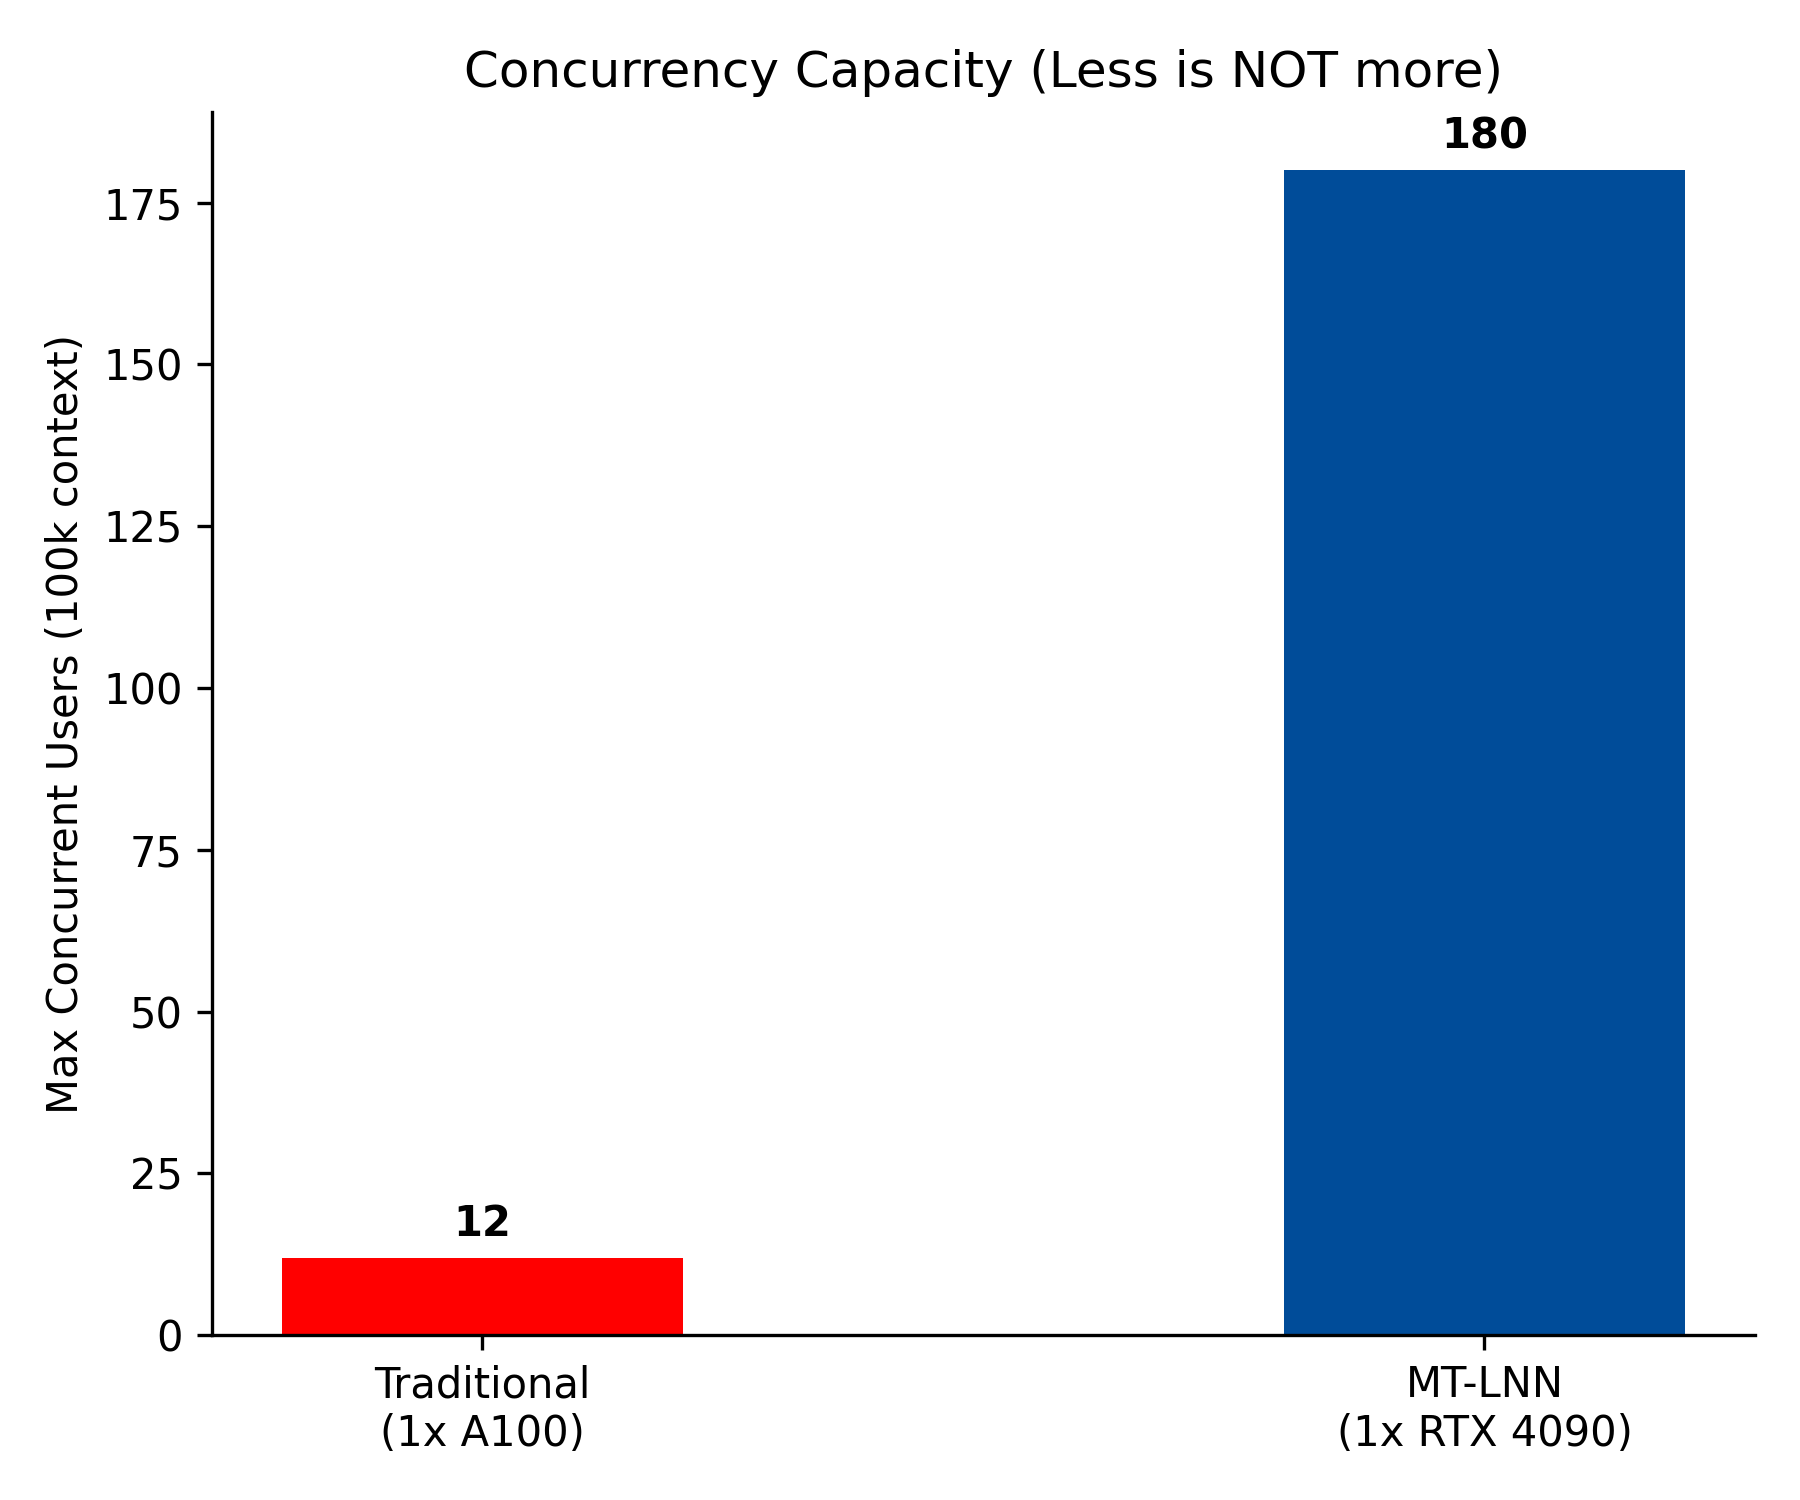
\includegraphics[width=\textwidth]{concurrency.png}
\end{column}
\begin{column}{0.5\textwidth}
\centering
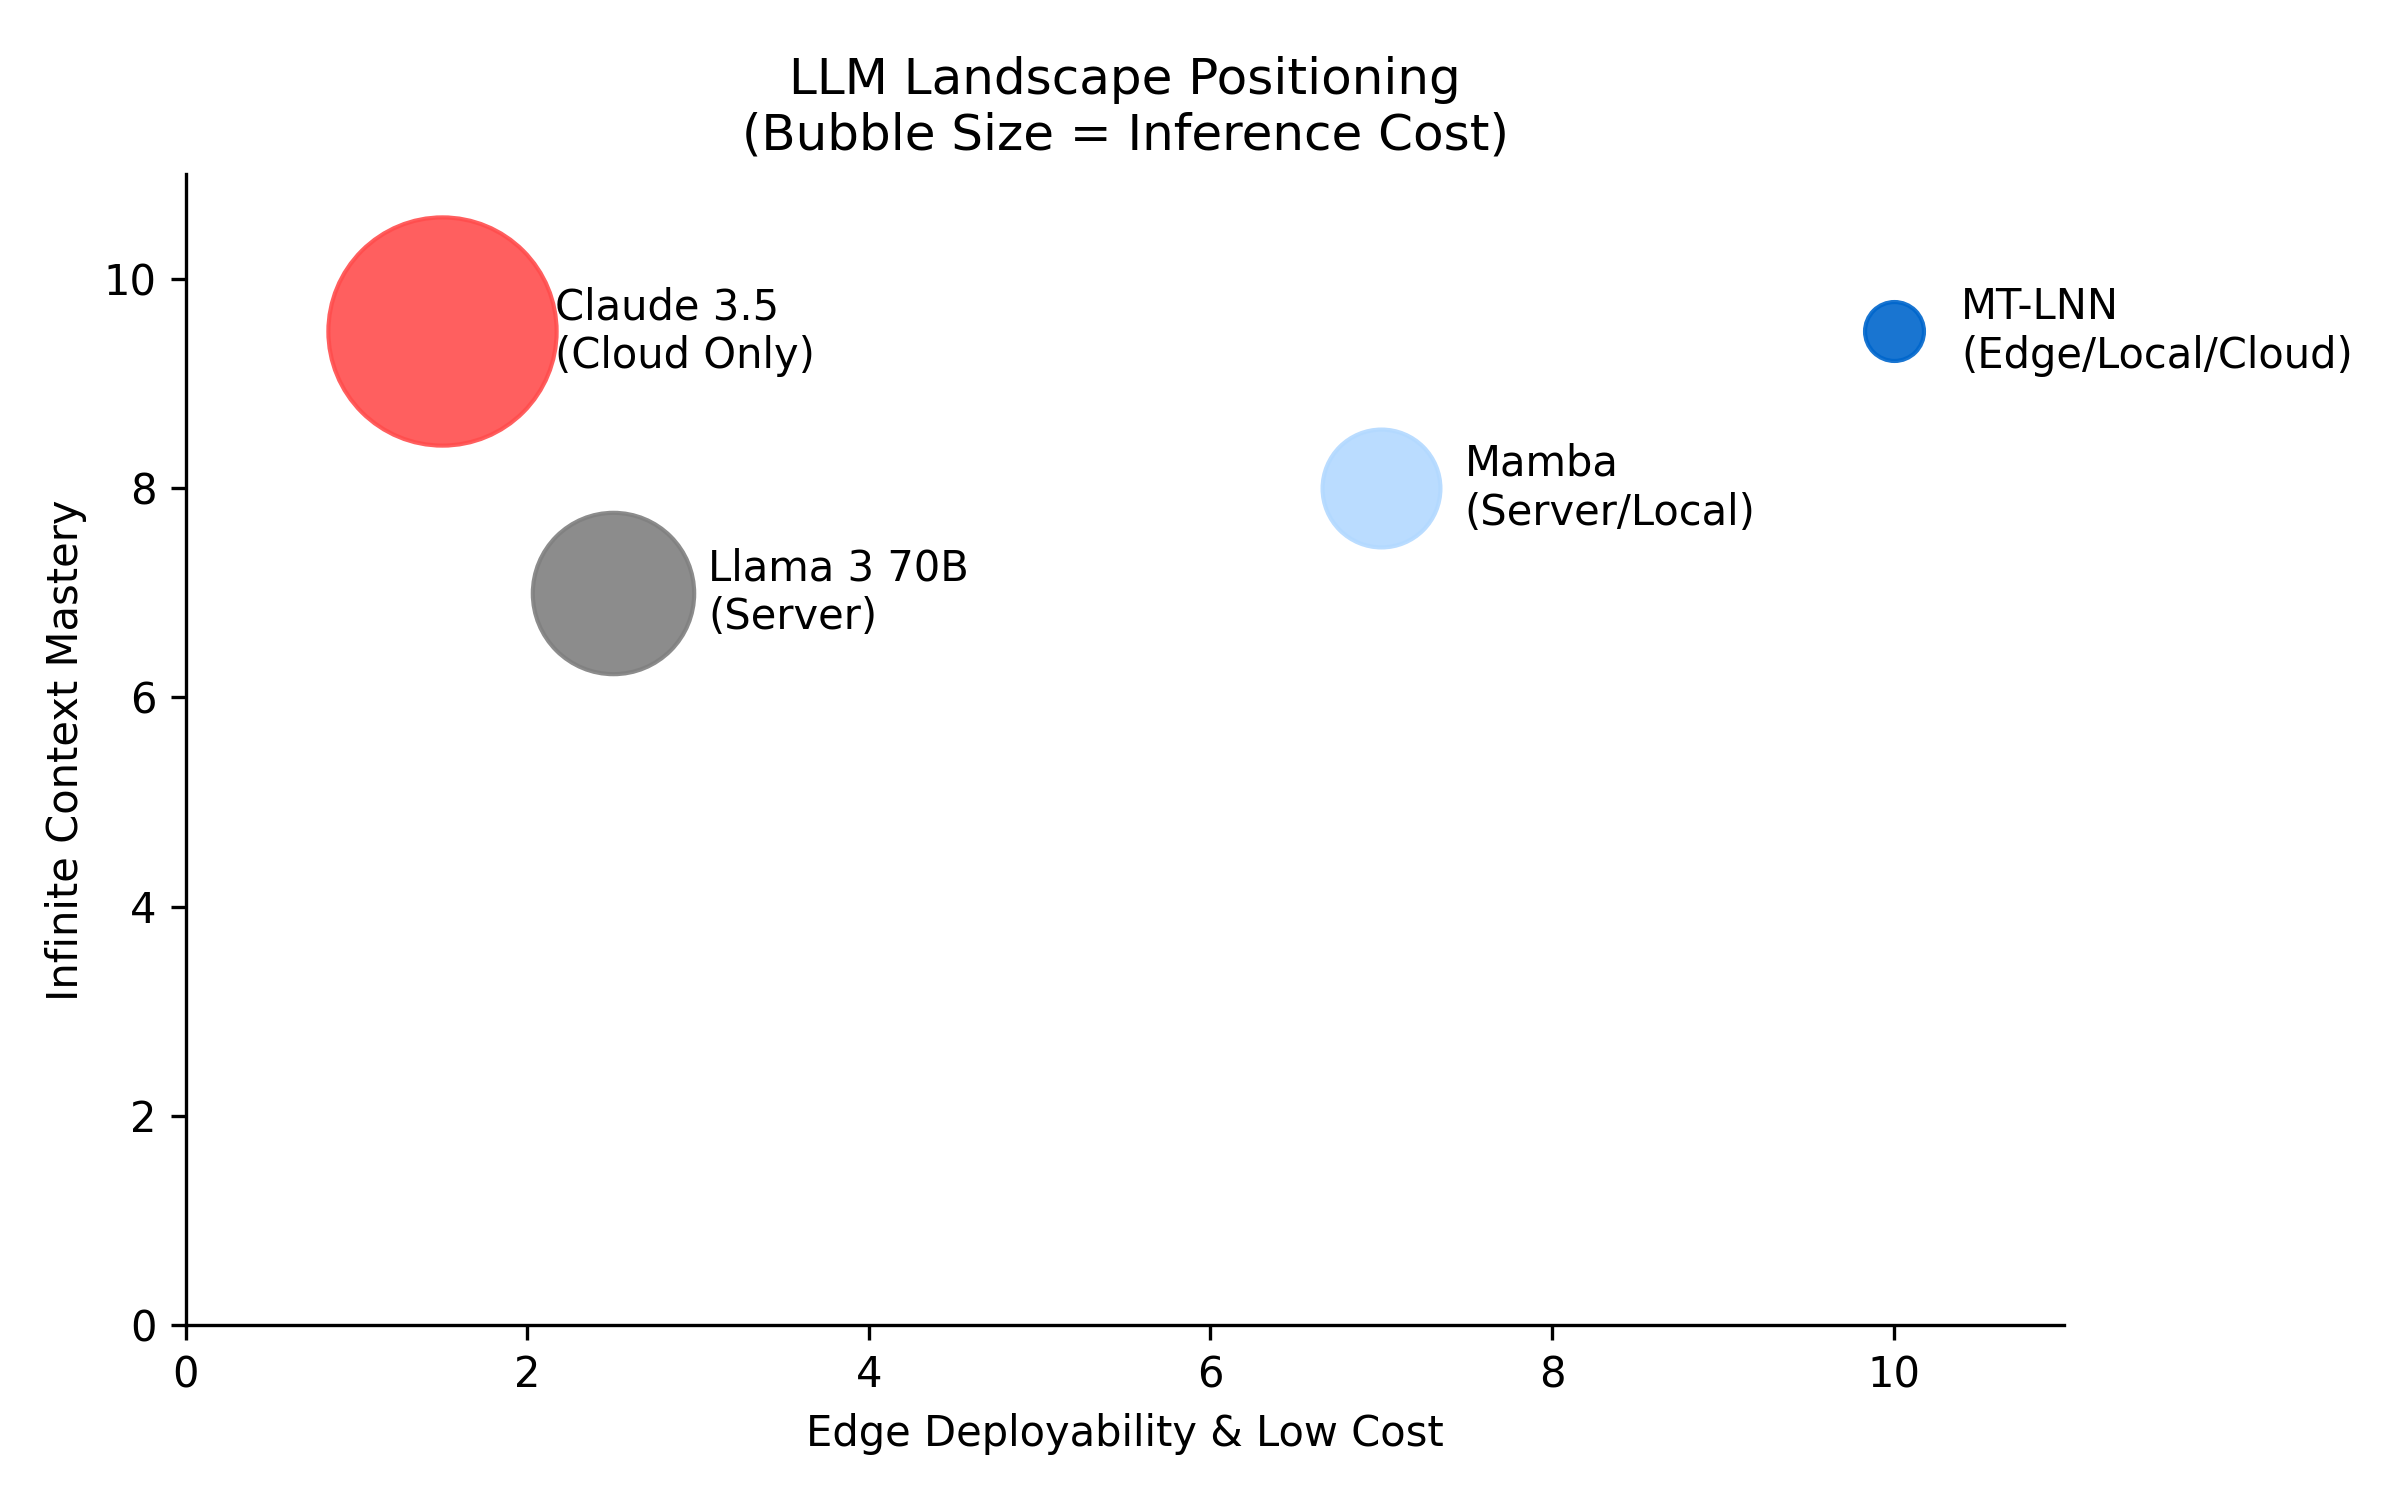
\includegraphics[width=\textwidth]{landscape.png}
\end{column}
\end{columns}
\end{frame}

\begin{frame}{Uncharted Territory 1: Edge \& IoT Devices}
\begin{itemize}
    \item \textbf{Solving the Hardware Bottleneck:} We are migrating advanced models directly into highly-constrained hardware: wearable AR glasses, native automotive local hubs, and flagship smartphones.
    \item \textbf{True ``Always-On'' Intelligence:} Our architecture supports continuous real-time audio/video processing. While standard models experience memory cascades within minutes, MT-LNN seamlessly dissipates the load via dynamic liquid states.
\end{itemize}
\end{frame}

\begin{frame}{Core Profit Center 2: B2B Enterprise Deadlocks}
\begin{itemize}
    \item \textbf{The Core Client Persona:} Top-tier law firms reviewing 1,000-page case files; hedge funds auditing 10,000 corporate annual reports; code reviewers untangling decades-old monolithic software structures.
    \item \textbf{100\% Pain-Point Overlap:} They suffer a trifecta of issues: (1) Need for massive document context, (2) Non-negotiable private local network deployments, (3) Unwillingness to buy \$200,000 GPU racks. MT-LNN dominates this exact intersection.
\end{itemize}
\end{frame}

\begin{frame}{Current Status: Million-Token RAG Demo}
\begin{itemize}
    \item \textbf{Not Just a Visionary Paper:} We have fully escaped the academic whiteboard. At this very moment, we possess a mature, running Python/Gradio UI integrating a natively functioning AI sandbox.
    \item \textbf{Ready to Deploy:} The codebase is fully containerized. It runs entirely offline on a standard PC or fits natively into an enterprise intranet. It is not an idea----it is a functional intelligence asset today.
\end{itemize}
\end{frame}

\begin{frame}{Product Roadmap (18-Month Vision)}
\begin{enumerate}
    \item \textbf{Phase 1: Validation (Current):} Utilizing small scale (1.5B components), we have achieved top-tier performance on long-context benchmarks and established an initial developer community.
    \vspace{0.4em}
    \item \textbf{Phase 2: Enterprise Deployment (Months 1-6):} Secure funding to train a native 7B enterprise model explicitly fine-tuned for dense RAG and local inference. Establish initial recurring B2B sales pipelines.
    \vspace{0.4em}
    \item \textbf{Phase 3: The A.G.I Checkmate (Months 6-18):} Scale to an H100 orbital cluster. Introduce multimodal processing and challenge the legacy Transformer architecture on a 100B+ parameter scale across global LLM arenas.
\end{enumerate}
\end{frame}

\begin{frame}{Team: The Architects Behind Awareness}
\begin{itemize}
    \item \textbf{Everest An -- Founder \& Core Architect} (AI Memory Expert)
    \vspace{0.5em}
    \item \textbf{Decentralized Infra \& Cryptography:} Former member of IPFS Athna, leading enterprise database construction deployment.
    \item \textbf{Top-Tier Investment \& Ecosystem:} Former Investment Manager at Outliers Fund. Led investments in L1 Chains (Dfinity, Harmony), Infra (Analog), and Smart Contract Audits (Quantstamp).
    \item \textbf{Global Engineering Prowess:} Multiple-time Champion at Global Ethereum Hackathons.
\end{itemize}
\end{frame}

\begin{frame}{Forward-Looking Pipeline (Scenario, Not Commitment)}
\footnotesize
\textit{All numbers below are planning scenarios contingent on the Seed / A round closing and architecture-team buildout. They are not signed contracts.}
\begin{itemize}\itemsep=0.3em
    \item \textbf{Year 1 (validation):} 5--10 paid design-partner PoCs in regulated B2B (Law / Finance / Defense). Goal: convert $\geq$ 3 to multi-year licenses; publish a 7B-scale checkpoint and an open benchmark report.
    \item \textbf{Year 2 (pipeline):} Convert design-partner cohort into qualified pipeline of \$5--10M annualized contract value. Launch the high-efficiency inference API as a second revenue stream once the on-prem motion is proven.
    \item \textbf{Year 4--5 (scale):} Aspirational \$50M+ ARR scenario assumes (a) on-prem motion has reached repeatable enterprise sales, (b) edge / always-on integrations have signed at least one chip-vendor partnership, (c) inference-cost advantage holds at 5--10$\times$ over Transformer baselines.
\end{itemize}
\end{frame}

\begin{frame}{The Ask: Seed / Series A}
\begin{columns}
\begin{column}{0.5\textwidth}
\textbf{Target Raise: \$3.5M}
\vspace{0.5em}
\begin{itemize}
    \item Fast-track 7B native foundational model training run.
    \item Build out the early B2B design-partner motion.
    \item \textbf{12-month milestones (non-revenue):}
    \begin{itemize}\footnotesize
        \item Sign LOIs / PoCs with $\geq$ 10 enterprise or research counterparties.
        \item Convert 3--5 into paid design partners (revenue not committed pre-close).
        \item Publish a production-grade 7B checkpoint + open benchmark report.
    \end{itemize}
\end{itemize}
\end{column}
\begin{column}{0.5\textwidth}
\textbf{Use of Funds:}
\begin{itemize}
    \item \textbf{50\% Compute \& Pre-Training:} H100 / A100 clusters for the 7B run.
    \item \textbf{30\% LNN Core Research:} Hire researchers extending continuous-time dynamics (LTC ODE), Orch-OR-inspired selection, and GWTB working memory. This is the differentiated moat.
    \item \textbf{20\% GTM \& Community:} Enterprise sales + OSS / paper / brand presence.
\end{itemize}
\end{column}
\end{columns}
\end{frame}

\begin{frame}{Where the Real Moat Lives}
\small
\begin{itemize}\itemsep=0.5em
    \item \textbf{Architecture originality (deepest layer):} MT-LNN itself --- continuous-time LTC ODE + Orch-OR-inspired selection + GWTB working memory --- is our original architecture, with a paper under submission. Architecture is the asset that cannot be quickly reproduced.
    \item \textbf{Reproducible training recipes \& cross-base experience:} adapter training data, hyperparameters, and ablation reports across Qwen-0.5B, Qwen-3B, and Llama bases are all committed to the repo. Even with the architecture in hand, a follow-on team needs months to reproduce this corpus of experience.
    \item \textbf{Self-built benchmark \& evaluation suite:} needle-in-a-haystack, selective-copy, O(1) memory stress tests, sparse-resonance ablations --- all self-designed, public, and reproducible.
    \item \textbf{OSS community + early design-partner flywheel:} code, weights, feedback loop shipped first. The same playbook Mamba and RWKV used to open a gap.
\end{itemize}
\end{frame}

\begin{frame}{Vision \& Conclusion}
\begin{itemize}
    \item \textbf{A New Scaling Path:} The traditional ``more compute, more scale'' Transformer paradigm faces diminishing marginal returns and severe memory constraints.
    \item \textbf{The Dynamic Liquid Advantage:} By transitioning to a fluid, continuous-time neural architecture, we bypass the ``Memory Wall'' holding back extensive AI enterprise integration.
    \item \textbf{Join the Next Wave:} You are backing a rigorously engineered system. We have the data, the verifiable codebase, and the highly efficient cost-basis necessary to reshape edge AI and enterprise deployments.
    \vspace{0.5em}
    \item \textit{Invest in Awareness. Invest in the Liquid Computing Paradigm Shift.}
\end{itemize}
\end{frame}

\begin{frame}{Contact Us \& Resources}
\begin{center}
    \LARGE \textbf{Awareness} \\
    \vspace{0.5em}
    \large Everest An -- Founder \& Core Architect \\
    \vspace{1.5em}
    \normalsize
    \textbf{Email:} everest9812@gmail.com \\
    \textbf{WeChat / Telegram:} EverestAn \\
    \vspace{1.5em}
    \small
    \textbf{Paper:} \url{https://huggingface.co/EverestAn/MT-LNN} \\
    \textbf{GitHub:} \url{https://github.com/everest-an/M1} \\
    \textbf{MT-LNN Demo:} \url{https://huggingface.co/spaces/EverestAn/AwarenessO1} \\
    \vspace{1.5em}
    \textit{Let's crush the AI Memory Wall together.}
\end{center}
\end{frame}

\end{document}

